\documentclass[12pt]{article}

\usepackage{a4wide}
\usepackage[utf8]{inputenc}

\usepackage{graphicx}

%\pagestyle{empty}

\begin{document}

\section*{Discrete Fourier Transform}

\noindent
Today's exercise is focused on implementation of the Discrete Fourier Transform (DFT).
In the upcoming lecture, we'll implement inverse transform.

\noindent
The Fourier Transform computes frequency spectrum of the given input image $f$.
This spectrum is denoted as $F$ (it's a complex matrix with dimensions of the input image).

\begin{equation}
    F(k, l) = \sum\limits_{m=0}^{M-1} \sum\limits_{n=0}^{N-1} f(m, n) \varphi_{k, l}(m, n)\,.
\end{equation}

\noindent
The basis $\varphi_{k, l}$ is defined as

\begin{equation}
    \varphi_{k, l}(m, n) = \frac{1}{\sqrt{MN}} e^{-i 2 \pi \left( \frac{mk}{M} + \frac{nl}{N} \right) }, k = 0, 1, \dots, M-1 \,\, \mathrm{a} \,\, l = 0, 1, \dots, N-1\,.
\end{equation}

\noindent
To compute the basis, it's advantageous to use Eulers formula $e^{ix} = \cos( x ) + i \sin( x )$.
Thanks to this equation, the solution is split into real and imaginary parts. More precisely:

\begin{equation}
    F(k, l) = R(k, l) + I(k, l)\, .
\end{equation}

\noindent
The spectrum amplituda $|F(k, l)|$ is computed as follows

\begin{equation}
    |F(k, l)| = \sqrt{ R^2(k, l) + I^2(k, l)}\, .
\end{equation}

\noindent
The phase $\Phi(k, l)$ is defined as follows

\begin{equation}
    \Phi(k, l) = \mathrm{arctg}\left( \frac{I(k, l)}{R(k, l)} \right)\, .
\end{equation}

\noindent
The power spectrum $P(k, l)$ may be computed easily as $ P(k, l) = |F(k, l)|^2$.

\noindent
You can display the power spectrum by logarithming the values of the spectrum and then normalizing values to the interval $\langle 0, 1\rangle$.
%
%
%Energetické spektrum signálu je možno zobrazit tak, že jej logaritmujeme a výsledné hodnoty normalizujeme do rozsahu $\langle 0, 1\rangle$.
\\
\\
\noindent
\textbf{Hint:} Use \texttt{double} data type to represent the input image, values of the frequency spectrum, and phase.
%{\textbf Hint:} Pracujete s datovým typem \texttt{double} pro reprezentaci vstupního obrazu, prvků frekvenčního spektra i fázového posuvu.

\section*{Expected Output}

\begin{center}
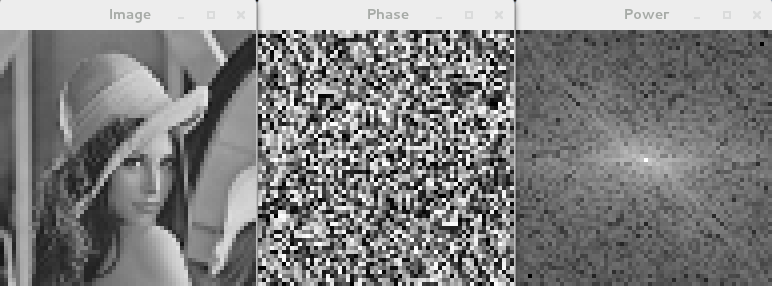
\includegraphics[width=0.8\textwidth]{result_images.png}
\end{center}

\end{document}

